% =============================================================================
% 2 Technische und normative Grundlagen
% =============================================================================
\section{Technische und normative Grundlagen}
\label{chap:technische_grundlagen}

Dieses Kapitel stellt die Grundlagen bereit, die für die Analyse des bestehenden
Erwärmungsprüfstands, die spätere Entwicklung des transformatorgestützten
Stellkonzepts sowie dessen Modellierung erforderlich sind. Im Mittelpunkt stehen
die normativen Randbedingungen der Erwärmungsprüfung, die elektrische und
thermische Beschreibung der Lastpfade sowie die für die spätere Regelung
benötigten Zusammenhänge. Eine allgemeine Darstellung von Schaltanlagen oder
Kontaktwerkstoffen ist nicht Gegenstand dieses Kapitels; entsprechende Aspekte
werden nur behandelt, soweit sie den untersuchten Prüfstand unmittelbar
beeinflussen.

% -----------------------------------------------------------------------------
% 2.1 Erwärmungsprüfung nach DIN EN IEC 61439
% -----------------------------------------------------------------------------
\subsection{Erwärmungsprüfung nach DIN EN IEC 61439}
\label{sec:erwaermungspruefung_norm}

Die Normenreihe DIN EN IEC~61439 enthält die Anforderungen an
Niederspannungs-Schaltgerätekombinationen. Teil~1 formuliert die allgemeinen
Festlegungen, ist jedoch nicht allein anzuwenden. Für die in dieser Arbeit
betrachteten Energie-Schaltgerätekombinationen werden die Festlegungen durch
Teil~2 ergänzt beziehungsweise konkretisiert
\autocite[Abschn.~1]{din_en_61439_1,din_en_61439_2}. Ein MCC-Feld wird damit im
Zusammenhang beider Normteile betrachtet.

Die Einhaltung der Bauartanforderungen wird durch den Bauartnachweis bestätigt.
Davon zu unterscheiden ist der Stücknachweis, der an jeder fertiggestellten
Schaltgerätekombination durchgeführt wird. Die Erwärmung gehört zu den im
Bauartnachweis zu verifizierenden Merkmalen. DIN EN IEC~61439-1 sieht hierfür
die Prüfung, die Ableitung von einer nachgewiesenen Referenzkonstruktion oder
eine Berechnung vor. Für den vorhandenen Prüfstand ist die experimentelle
Verifikation durch Strombelastung maßgebend
\autocite[Abschn.~3.9.1, 3.9.2 und 10.10]{din_en_61439_1}.

Ziel der Erwärmungsprüfung ist der Nachweis, dass die bei festgelegter Belastung
entstehenden Temperaturen beziehungsweise Übertemperaturen die zulässigen
Grenzen nicht überschreiten. Die Übertemperatur ist die Differenz zwischen der
Temperatur des betrachteten Punktes und der Umgebungstemperatur:

\begin{equation}
  \Delta\vartheta = \vartheta - \vartheta_\mathrm{U}.
  \label{eq:uebertemperatur}
\end{equation}

Die zulässige Übertemperatur ist kein einheitlicher Wert für die gesamte
Schaltgerätekombination. Sie hängt unter anderem von der Art des Betriebsmittels,
dem Werkstoff und der Funktion des betrachteten Messpunktes ab. Deshalb müssen
Messstellen und Grenzwerte aus der konkreten Nachweisaufgabe abgeleitet werden
\autocite[Abschn.~9.2 und Tab.~6]{din_en_61439_1}.

Für die Prüfung einer vollständigen Schaltgerätekombination ist eine
repräsentative Aufstellung einschließlich der vorgesehenen elektrischen
Verbindungen herzustellen. Die Stromkreise werden mit den für den Nachweis
festgelegten Strömen belastet; die Temperaturen sind an den relevanten Stellen
und die Umgebungstemperatur gleichzeitig zu erfassen. Der thermische
Beharrungszustand gilt als erreicht, wenn sich die Temperaturänderung an allen
Messstellen einschließlich der Umgebungstemperatur auf höchstens
\SI{1}{\kelvin\per\hour} verringert hat
\autocite[Abschn.~10.10.2.3.1]{din_en_61439_1}.

Bei der Prüfung durch Strombelastung ist außerdem zwischen dem Mittelwert der
tatsächlichen Außenleiterströme am Einspeisepunkt und der Abweichung der
einzelnen Außenleiter zu unterscheiden. Der Mittelwert ist auf
\SIrange{100}{103}{\percent} des vorgesehenen Prüfstroms einzustellen; jeder
Außenleiter darf vom Mittelwert um höchstens \SI{5}{\percent} abweichen
\autocite[Abschn.~10.10.2.3.1]{din_en_61439_1}. Diese Vorgabe ist daher nicht
gleichbedeutend mit der pauschalen Forderung, jeder beliebige Modulstrom müsse
zu jedem Zeitpunkt zwischen \SI{100}{\percent} und \SI{105}{\percent} seines
Bemessungsstroms liegen. Welche Teilströme für den konkreten Nachweis einzustellen
und zu überwachen sind, ergibt sich aus der gewählten Prüfanordnung und dem
Nachweisziel.

Für diese Arbeit folgen daraus drei wesentliche Randbedingungen: Erstens müssen
die relevanten Ströme über die lange Dauer bis zum thermischen
Beharrungszustand ausreichend stabil gehalten werden. Zweitens ist neben dem
übergeordneten Einspeisestrom die Verteilung auf die gleichzeitig belasteten
Abgänge zu beachten. Drittens muss eine Änderung der Stromeinstellung ohne
unzulässige Beeinflussung der Temperaturmessung und unter Einhaltung der
betrieblichen Sicherheitsvorgaben möglich sein.

% -----------------------------------------------------------------------------
% 2.2 MCC-Feld und zu prüfende Abgangseinheiten
% -----------------------------------------------------------------------------
\subsection{MCC-Feld und zu prüfende Abgangseinheiten}
\label{sec:mcc_feld_grundlagen}

Ein Motor Control Center (MCC) ist eine Niederspannungs-Schaltgerätekombination,
in der mehrere Abgangseinheiten zur Versorgung und zum Schutz elektrischer
Verbraucher zusammengefasst sind. Die Energie wird über Haupt- und
Verteilschienensysteme zu den einzelnen Abgangseinheiten geführt. Für eine
Erwärmungsprüfung ist dabei nicht nur der Gesamtstrom des Feldes relevant. Die
Verlustleistung entsteht verteilt in Schienen, Verbindungsstellen, Schalt- und
Schutzgeräten sowie in den Anschlussleitungen der einzelnen Abgänge. Die
Stromaufteilung bestimmt somit, welche Bereiche der Schaltgerätekombination
thermisch beansprucht werden.

Das im Rahmen dieser Arbeit betrachtete Prüffeld besitzt zwölf gleichzeitig zu
betrachtende Abgänge. Die vorgesehene Konfiguration ist in
Tabelle~\ref{tab:pruefkonfiguration_mcc} zusammengefasst. Die Summe der
vorgegebenen Abgangsströme beträgt rechnerisch \SI{1730}{\ampere}. Die Werte
beschreiben die projektbezogene Prüfanordnung und sind nicht als allgemeine
Bemessung eines MCC-Feldes zu verstehen
\autocite{rj_mcc_pruefkonfiguration_2026}.

\begin{table}[htbp]
  \centering
  \caption{Projektbezogene Konfiguration der zu prüfenden Abgangseinheiten}
  \label{tab:pruefkonfiguration_mcc}
  \begin{tabular}{lrrr}
    \toprule
    Abgangsgröße & Anzahl & Strom je Abgang & Teilsumme \\
    \midrule
    A-Modul   & 6 & \SI{40}{\ampere}  & \SI{240}{\ampere} \\
    B-Modul   & 3 & \SI{70}{\ampere}  & \SI{210}{\ampere} \\
    1er-Modul & 1 & \SI{250}{\ampere} & \SI{250}{\ampere} \\
    2er-Modul & 1 & \SI{400}{\ampere} & \SI{400}{\ampere} \\
    3er-Modul & 1 & \SI{630}{\ampere} & \SI{630}{\ampere} \\
    \midrule
    Gesamt    & 12 & -- & \SI{1730}{\ampere} \\
    \bottomrule
  \end{tabular}
\end{table}

Die starke Spreizung zwischen \SI{40}{\ampere} und \SI{630}{\ampere} ist für
die spätere Optimierung besonders bedeutsam. Ein gemeinsames Stellglied kann
zwar die Einspeisung des gesamten Feldes verändern, es kann jedoch nicht ohne
Weiteres die unterschiedlichen Driftanteile aller zwölf Lastpfade einzeln
ausgleichen. Die konstruktive Ausführung des Feldes und der genaue Energiepfad
werden deshalb in Kapitel~\ref{chap:analyse_pruefstand} anhand des bestehenden
Prüfstands untersucht.

% -----------------------------------------------------------------------------
% 2.3 Elektrische Verlustleistung und temperaturabhängiger Widerstand
% -----------------------------------------------------------------------------
\subsection{Elektrische Verlustleistung und temperaturabhängiger Widerstand}
\label{sec:verlustleistung_temperaturkoeffizient}

Die Erwärmung eines stromdurchflossenen Leiters entsteht im betrachteten Modell
im Wesentlichen durch ohmsche Verluste. Für einen Gleichstrom beziehungsweise
für Effektivwerte bei annähernd ohmscher Belastung gilt

\begin{equation}
  P_\mathrm{el} = U I = I^2 R = \frac{U^2}{R}.
  \label{eq:elektrische_verlustleistung}
\end{equation}

Bei einem dreiphasigen System ist die gesamte Verlustleistung als Summe der
Leistungen der drei Außenleiter beziehungsweise der einzelnen Lastpfade zu
bilden. Die Schreibweise in Gleichung~\ref{eq:elektrische_verlustleistung}
bezieht sich daher jeweils auf den betrachteten Ersatzpfad.

Der Widerstand eines homogenen Leiters kann über den spezifischen elektrischen
Widerstand $\rho$, die wirksame Leiterlänge $l$ und den Querschnitt $A$
beschrieben werden:

\begin{equation}
  R = \rho\,\frac{l}{A}.
  \label{eq:widerstand_geometrie}
\end{equation}

Diese Beziehung erklärt das Wirkprinzip der im Prüfstand eingesetzten
verstellbaren V2A-Lastwiderstände: Durch das Versetzen der Anschluss- oder
Kurzschlussbrücke wird die wirksame Leiterlänge und damit der Widerstand des
jeweiligen Lastpfades verändert.

Für einen begrenzten Temperaturbereich kann der Widerstand metallischer Leiter
linear angenähert werden. Bezogen auf \SI{20}{\degreeCelsius} ergibt sich

\begin{equation}
  R(\vartheta) = R_{20}\left[1 + \alpha_{20}
  \left(\vartheta-\SI{20}{\degreeCelsius}\right)\right].
  \label{eq:widerstand_temperatur}
\end{equation}

Dabei bezeichnet $R_{20}$ den Widerstand bei \SI{20}{\degreeCelsius} und
$\alpha_{20}$ den zugehörigen Temperaturkoeffizienten
\autocite[Abschn.~2.1.4]{plassmann_formeln}. Für V2A ist kein universeller
Koeffizient anzusetzen, da die Bezeichnung eine Werkstoffgruppe umfasst und der
konkrete Wert von Legierung und Zustand abhängt. Der im Simulationsmodell
verwendete Parameter muss daher aus dem eingesetzten Werkstoff, einem
Herstellerwert oder einer Messung abgeleitet und in
Kapitel~\ref{chap:modellbildung} dokumentiert werden.

Aus den Gleichungen~\ref{eq:elektrische_verlustleistung} und
\ref{eq:widerstand_temperatur} folgt, dass die Rückwirkung der Erwärmung von der
elektrischen Randbedingung abhängt. Bei näherungsweise konstanter Spannung sinken
mit steigendem Widerstand sowohl Strom als auch Verlustleistung:

\begin{equation}
  I = \frac{U}{R(\vartheta)}, \qquad
  P_\mathrm{el} = \frac{U^2}{R(\vartheta)}.
  \label{eq:konstante_spannung}
\end{equation}

Bei eingeprägtem Strom steigt die Verlustleistung dagegen gemäß
$P_\mathrm{el}=I^2R(\vartheta)$. Der reale Prüfstand liegt zwischen diesen
idealen Grenzfällen: Die gemeinsame Quelle, ihre Innenimpedanz und die parallel
betriebenen Lastpfade koppeln die einzelnen Abgangsströme miteinander. Diese
Kopplung ist die zentrale Ursache dafür, dass ein zentral geregelter Gesamtstrom
keine eindeutige Aussage über jeden einzelnen Abgangsstrom erlaubt.

% -----------------------------------------------------------------------------
% 2.4 Thermisches Verhalten und RC-Ersatzmodell
% -----------------------------------------------------------------------------
\subsection{Thermisches Verhalten und RC-Ersatzmodell}
\label{sec:thermisches_rc_grundlagen}

Die einem Körper zugeführte Wärmeenergie $Q$ ergibt sich aus der zeitlichen
Integration des Wärmestroms $\dot Q$:

\begin{equation}
  Q(t)=\int_{t_0}^{t}\dot Q(\tau)\,\mathrm{d}\tau,
  \qquad
  \dot Q(t)=\frac{\mathrm{d}Q}{\mathrm{d}t}.
  \label{eq:waermeenergie_waermestrom}
\end{equation}

Für ein konzentriertes thermisches Modell wird die Wärmespeicherfähigkeit eines
Bauteils durch die thermische Kapazität $C_\mathrm{th}$ und die Wärmeabgabe an
die Umgebung durch den thermischen Widerstand $R_\mathrm{th}$ beschrieben. Die
elektrische Analogie ist in Abbildung~\ref{fig:thermisches_rc_grundmodell}
dargestellt. Temperaturdifferenz, Wärmestrom, thermische Kapazität und
thermischer Widerstand entsprechen dabei Spannung, Strom, elektrischer
Kapazität und elektrischem Widerstand.

\begin{figure}[H]
    \centering
    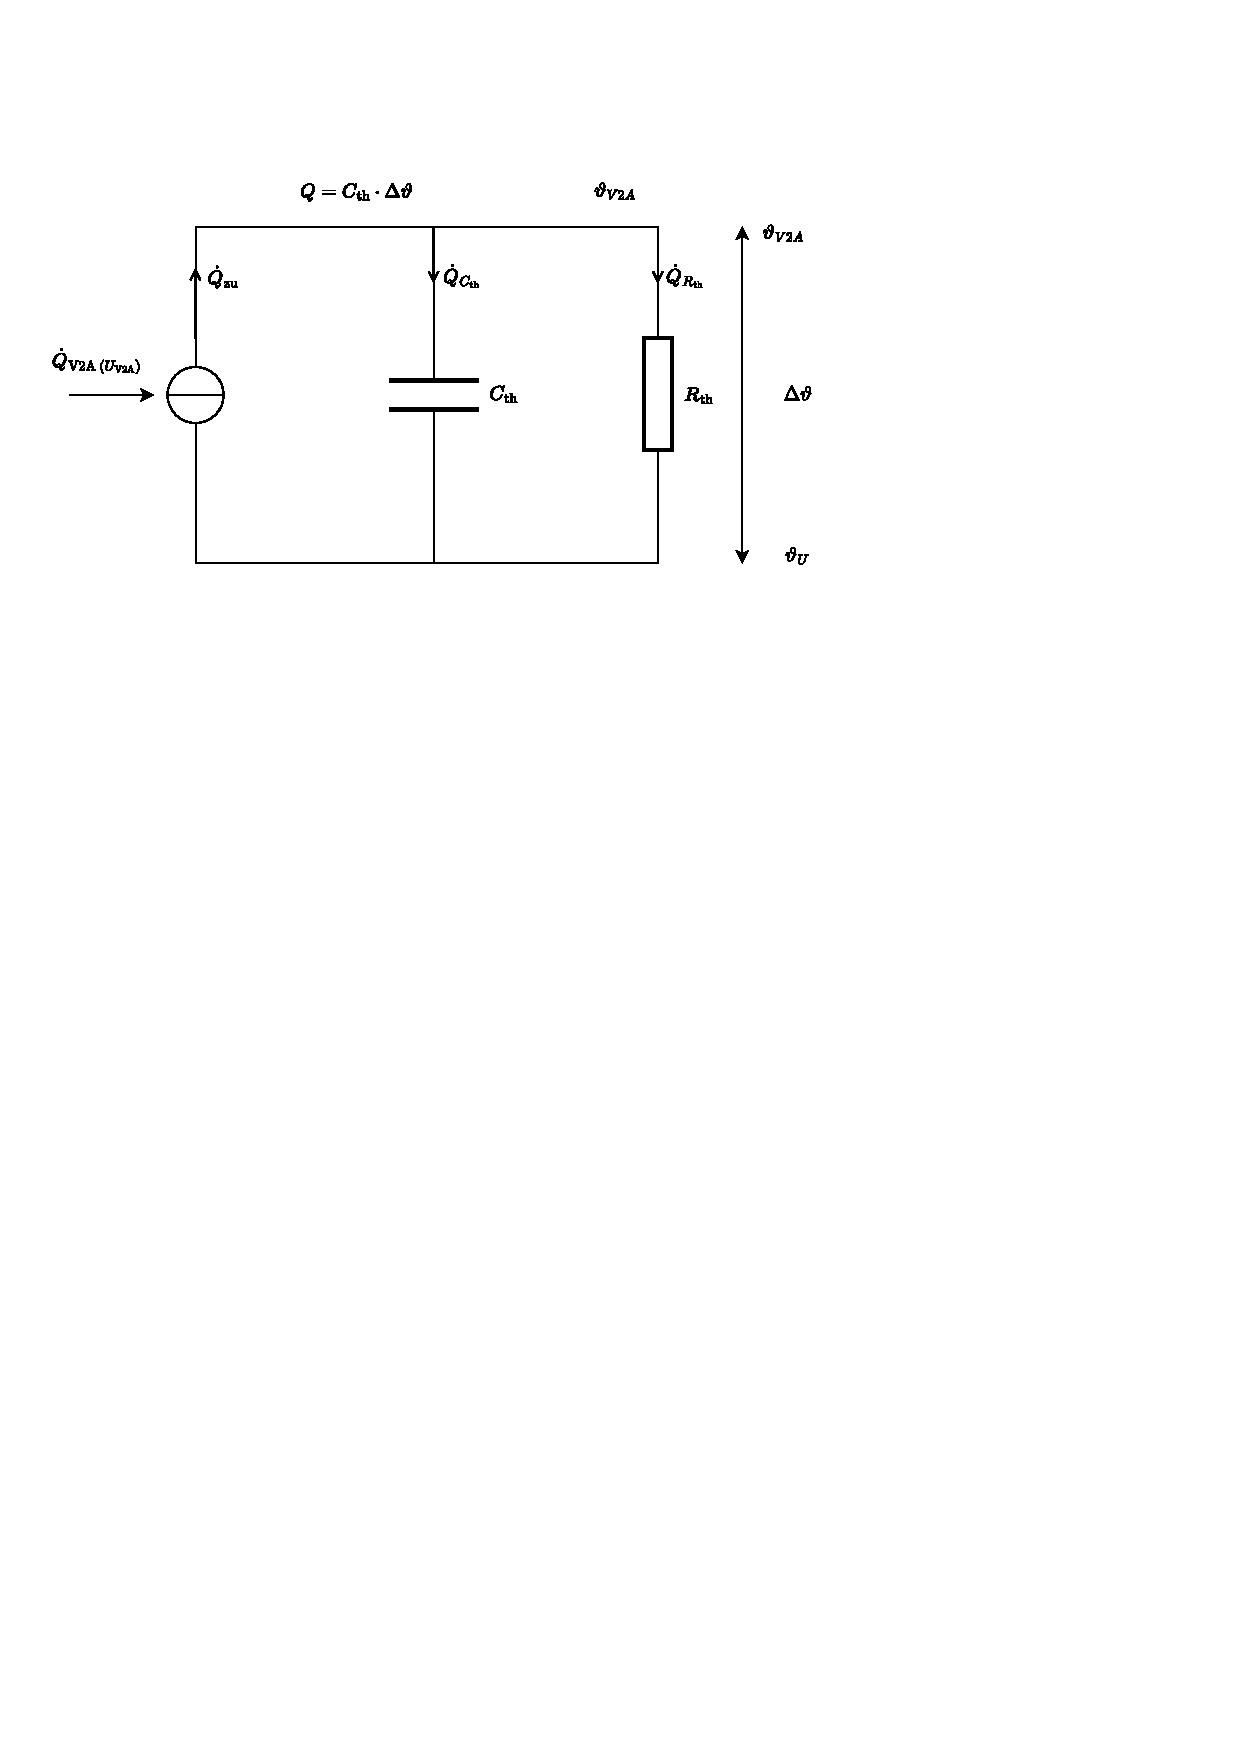
\includegraphics[width=0.90\textwidth]{03_Ressourcen/drawio/ESB_thermisches_ersatzschaltbild_drift.pdf}
    \caption{Thermisches RC-Ersatzschaltbild des V2A-Lastwiderstands}
    \label{fig:thermisches_rc_grundmodell}
\end{figure}

Mit $\Delta\vartheta=\vartheta-\vartheta_\mathrm{U}$ lautet die Energiebilanz
des Modells

\begin{equation}
  C_\mathrm{th}\frac{\mathrm{d}\Delta\vartheta}{\mathrm{d}t}
  = P_\mathrm{el}(t)-\frac{\Delta\vartheta(t)}{R_\mathrm{th}}.
  \label{eq:thermische_dgl_grundlage}
\end{equation}

Für eine konstante Verlustleistung $P_\mathrm{el}$ ergibt sich die stationäre
Übertemperatur zu

\begin{equation}
  \Delta\vartheta_\infty=P_\mathrm{el}R_\mathrm{th}.
  \label{eq:stationaere_uebertemperatur}
\end{equation}

Die thermische Zeitkonstante beträgt

\begin{equation}
  T_\mathrm{th}=R_\mathrm{th}C_\mathrm{th}.
  \label{eq:thermische_zeitkonstante}
\end{equation}

Nach einem Leistungssprung von null auf $P_\mathrm{el}$ nähert sich die
Übertemperatur bei einer Anfangsübertemperatur $\Delta\vartheta_0$ gemäß

\begin{equation}
  \Delta\vartheta(t)=\Delta\vartheta_\infty
  +\left(\Delta\vartheta_0-\Delta\vartheta_\infty\right)
  \mathrm{e}^{-t/T_\mathrm{th}}.
  \label{eq:pt1_sprungantwort_thermisch}
\end{equation}

exponentiell dem Endwert an. Das Modell besitzt damit PT1-Verhalten
\autocite{Griesinger_Waermemanagement}
\autocite[Kap.~2 und 6]{rossmann2020magnetismus}.
Die Zusammenfassung von Wärmeleitung, Konvektion und Strahlung in einem
konstanten $R_\mathrm{th}$ ist eine Linearisierung. Sie ist für die Untersuchung
des grundsätzlichen Driftverhaltens zweckmäßig, muss jedoch durch Grenzfälle und
Vergleiche plausibilisiert werden. Die Herleitung über Differentialgleichung
und Laplace-Transformation sowie die elektrothermische Rückkopplung werden erst
in Kapitel~\ref{chap:modellbildung} vollständig ausgearbeitet.

% -----------------------------------------------------------------------------
% 2.5 Transformator und Impedanztransformation
% -----------------------------------------------------------------------------
\subsection{Transformator und Impedanztransformation}
\label{sec:transformator_impedanztransformation}

Ein Transformator überträgt elektrische Energie elektromagnetisch zwischen
Wicklungen. Bei einem Transformator mit getrennten Wicklungen besteht dabei
zusätzlich eine galvanische Trennung. Für den idealen
Zweiwicklungstransformator wird das Übersetzungsverhältnis $\ddot{u}$ über die
Windungszahlen definiert:

\begin{equation}
  \ddot{u}=\frac{N_1}{N_2}=\frac{U_1}{U_2}
  =\frac{I_2}{I_1}.
  \label{eq:transformator_uebersetzung}
\end{equation}

Eine an der Sekundärseite angeschlossene Impedanz $Z_2$ erscheint auf der
Primärseite mit

\begin{equation}
  Z'_2=\ddot{u}^{2} Z_2.
  \label{eq:impedanztransformation}
\end{equation}

Die quadratische Impedanztransformation ist für das Optimierungskonzept
entscheidend. Eine Widerstandsänderung auf einer Seite des Transformators wirkt
mit dem Quadrat des Übersetzungsverhältnisses auf die andere Seite zurück. Auf
diese Weise kann ein Stellwiderstand in einem Bereich angeordnet werden, in dem
die zu beherrschenden Ströme deutlich kleiner als die primären Modulströme sind.
Reale Transformatoren weisen zusätzlich Wicklungswiderstände,
Streuinduktivitäten, Magnetisierungsstrom und Verluste auf. Welche dieser
Effekte im späteren Modell berücksichtigt werden, richtet sich nach ihrem
Einfluss auf die untersuchte Stromnachführung
\autocite[Kap.~6]{rossmann2020magnetismus}.

% -----------------------------------------------------------------------------
% 2.6 Grundlagen der Stromregelung
% -----------------------------------------------------------------------------
\subsection{Grundlagen der Stromregelung}
\label{sec:grundlagen_stromregelung}

Eine Regelung erfasst die Regelgröße fortlaufend und führt sie durch Rückkopplung
an einen vorgegebenen Sollwert heran. In der in
Abbildung~\ref{fig:regelkreis_grundstruktur} gezeigten Grundstruktur wird der
Istwert $y(t)$ über das Messglied zurückgeführt und mit dem Sollwert $w(t)$
verglichen. Aus der Regeldifferenz

\begin{equation}
  e(t)=w(t)-y(t)
  \label{eq:regeldifferenz}
\end{equation}

bildet der Regler die Stellgröße $u(t)$. Das Stellglied setzt diese in eine
physikalische Änderung der Regelstrecke um. Störgrößen $z(t)$ können unmittelbar
auf die Regelstrecke wirken
\autocite[Kap.~2]{rossmann2020magnetismus}.

\begin{figure}[H]
    \centering
    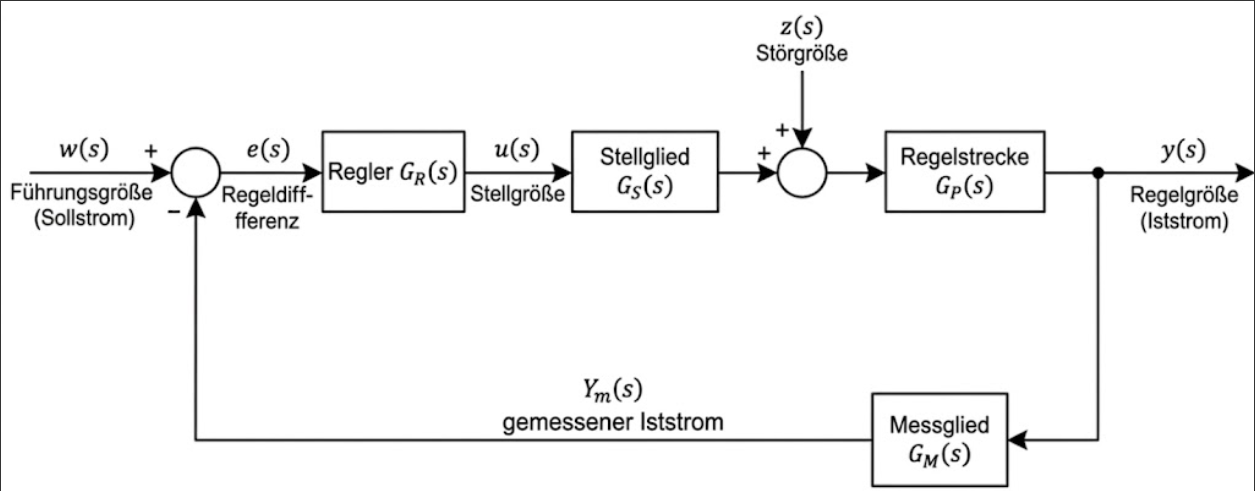
\includegraphics[width=0.95\textwidth]{03_Ressourcen/pic/regelkreis_stromregelung.png}
    \caption{Grundstruktur des geschlossenen Regelkreises zur Nachführung
    eines Modulstroms (eigene Darstellung in Anlehnung an
    \textcite[Kap.~2]{rossmann2020magnetismus})}
    \label{fig:regelkreis_grundstruktur}
\end{figure}


Auf den Prüfstand übertragen ist der Strom eines Abgangs die Regelgröße. Die
thermisch bedingte Widerstandsänderung wirkt als langsam veränderliche Störung.
Das Stellglied muss den Strom innerhalb seines Stellbereichs korrigieren können,
ohne Instabilität oder unzulässige Wechselwirkungen mit den übrigen Abgängen zu
verursachen. Ein Integralanteil ist grundsätzlich geeignet, eine bleibende
Regelabweichung bei konstanten Störungen abzubauen; seine konkrete Auslegung ist
jedoch erst nach Kenntnis von Strecke, Stellgeschwindigkeit, Messauflösung und
Kopplung möglich.

Bei zwölf gleichzeitig betriebenen Abgängen liegt ein Mehrkanalsystem vor. Sind
die Kanäle über die gemeinsame Quelle gekoppelt, verändert eine Stellhandlung
nicht ausschließlich den zugehörigen Abgang. Die spätere Regelungsstrategie muss
daher sowohl die lokale Regelabweichung als auch die Wirkung auf den
übergeordneten Strompfad berücksichtigen. Kapitel~\ref{chap:analyse_pruefstand}
untersucht zunächst, wie diese Kopplung im bestehenden Prüfstand entsteht.